\documentclass{article}
\date{February 2019}
\author{Joe Singleton}
\title{
    Notes on theory of truth discovery algorithms
}

% Packages:
\usepackage{amsmath}
\usepackage{amsthm}
\usepackage{caption}
\usepackage{cite}
\usepackage[top=2cm, bottom=2cm, left=3cm, right=3cm]{geometry}
\usepackage{graphicx}
\usepackage{hyperref}
\usepackage{multicol}
\usepackage{tgbonum}  % For cool font
\usepackage{xcolor}

\graphicspath{ {./images/} }

% Settings
\hypersetup{
	colorlinks,
	citecolor={blue!80!black},
	urlcolor={blue!80!black},
	linkcolor={blue!80!black}
}

% Maths environments
\theoremstyle{definition}
\newtheorem{definition}{Definition}
\theoremstyle{plain}
\newtheorem{axiom}{Axiom}
\theoremstyle{plain}
\newtheorem{remark}{Remark}
\theoremstyle{remark}
\newtheorem{notation}{Notation}

% Commands
\newcommand{\todo}[1] {
    \textcolor{red}{
        \textbf{TODO:} #1
    }
}
\renewcommand{\S}{\mathcal{S}}  % Note: overrides existing command
\renewcommand{\O}{\mathcal{O}}  % Note: overrides existing command
\newcommand{\F}{\mathcal{F}}
\newcommand{\sle}{\le}
\newcommand{\fle}{\preceq}
\newcommand{\sge}{\ge}
\newcommand{\fge}{\succeq}
\newcommand{\tdn}{truth-discovery network}
\newcommand{\tda}{truth-discovery algorithm}

\begin{document}
\maketitle
% \begin{multicols}{2}

\section{Frameworks for truth-discovery used in existing literature}
\label{sec:existing_frameworks}

\subsection{Li et. al. survey}
\label{sec:li}

A 2015 survey by Li et. al. {\cite{li_survey}} defines truth-discovery as
follows.

\begin{itemize}
\item We have a set of sources $\S$, and a set of objects $\O$
\item Each source $s$ claims a value $v_{o}^{s}$ for some objects $o$ (not
necessarily \emph{all} objects)
\item Truth-discovery: compute a \emph{source weight} $w_s$ for each source,
and compute `truth values' $v_{o}^{*}$ for each object $o$
\item \emph{Single truth assumption}: there is exactly one true value for each
object. This may not always hold (e.g. consider which actors star in a film)
\end{itemize}

\subsection{Gupta and Han survey}
\label{sec:gupta}

From \cite{gupta_han_survey}, slightly re-phrased by me (e.g. paper calls
sources `providers', denotes confidence by $s$\ldots)

\begin{itemize}
\item Set of sources $\S$, objects $\O$
\item Each object $o$ has as associated set of \emph{facts} $F_o$. Write
$\F = \bigcup_{o \in \O}F_o$
\item Sources \emph{provide} facts about objects. They may provide facts about
multiple objects, but only one fact per object
\item Could be formalised similar to \ref{sec:li} as follows: $f_o^s \in F_o$
is the fact provided by source $s$ for object $o$, defined for a subset of $\O$
\item Truth-discovery: compute \emph{source trusts} $t_s$ for each source $s$,
and \emph{fact confidence} $c_f$ for each fact $f$
\end{itemize}

Note that general set up is more or less equivalent to in \ref{sec:li}: facts
replace values. However the definition of a truth-discovery algorithm is
different: here each fact is given a confidence score, whereas in \ref{sec:li}
we only find the most believable fact for each object.

If each fact is given a confidence score then it is simple to find most
believed fact for each object by taking the fact with highest confidence.

\subsection{Latent Dirichlet Truth Discovery}
\label{sec:ldt}

The method proposed in \cite{zhang_qi_tang} is similar to both above approaches:

\begin{itemize}
\item Set of sources $\S$, objects $\O$, facts $F_o$ for each $o \in \O$
\item Each source $s$ makes claim $\texttt{Cl}_o(s) \in F_o \cup
\{\oslash\}$ for the true fact for object $o$, where $\oslash$ is special
symbol to indicate no claim is made
\item Each source has a \emph{trustworthy component} and \emph{untrustworthy
component}
\item Truth-discovery:
    \begin{itemize}
    \item Compute probability that each fact $f$ is the true fact for its
    associated object (i.e. confidence in each fact?)
    \item Compute trustworthy and untrustworthy amounts in each source
    (trustworthy amount can be considered source trustworthiness, comparable to
    other approaches)
    \end{itemize}
\end{itemize}

\subsection{Pasternack and Roth}
\label{sec:past}

In \cite{pasternack}:

\begin{itemize}
\item Set of sources $\S$, each with a set of claims $C_s$ ($s \in \S$). Write
$\mathcal{C} = \bigcup_{s \in \S}{C_s}$
\item Each claim $c$ has \emph{mutual exclusion} set $M_c \subseteq
\mathcal{C}$: only one claim in each $M_c$ is true. Note that $c \in M_c$
\item Truth-discovery: compute source trusts $t_s$ and claim beliefs $b_c$
\end{itemize}

This is essentially the same as \ref{sec:gupta}, if we let each mutual
exclusion set be called an object, rename claims to facts, and the facts
provided by source $s$ are simply those in $C_s$. Something like the following.
$$
\O = \{M_c : c \in \mathcal{C}\},
\quad
F_{M_c} = M_c
$$

The only slight problem is that under this mapping a fact (\ref{sec:gupta}
sense) may be related to multiple objects, e.g. if $c \in M_{c'}$ but $M_c \ne
M_{c'}$.

\subsection{Galland et. al algorithms}
\label{sec:galland}

Several algorithms are proposed in \cite{galland}, and each uses the following
scheme, which is initially quite different from those above (again, slightly
re-phrased by me in places):

\begin{itemize}
\item Set of sources $\S$, facts $\F$, and the \emph{real world}
$W: \F \rightarrow \{\texttt{True}, \texttt{False}\}$
\item Each source $s$ is a partial mapping $\F \rightarrow
\{\texttt{True}, \texttt{False}\}$
\item Each source $s$ has an \emph{error factor} $\epsilon(s) \in [0, 1]$ (?)
that represents the likeliness of $s$ making a mistake on the truth value of
any given fact
\item Set of \emph{queries} $\mathcal{Q}$. Each fact $f$ has a \emph{reference
query} $ref(f) \in \mathcal{Q}$ (imagine that $q\in\mathcal{Q}$ is a question,
and $f$ answers the question in some way). Any query has exactly one true fact.
Formally, for each query $q$, let $F_q = \{f \in \F : ref(f) = q\}$.
For each $q$ there is exactly one $f \in F_q$ with $W(f) = \texttt{True}$ \item
Truth-discovery: compute source error factors $\epsilon(s)$, and an estimate
for the real world $W$ given as a mapping $\F \rightarrow [0, 1]$ where 1
represents true and 0 represents false.
\end{itemize}

Some important differences here:
\begin{itemize}
\item Sources may claim a fact is \emph{false}, which is not possible in the
other approaches
\item Objects are not first-class citizens
\item Notion of queries. The set of queries (along with the reference query for
each fact) is not given as input to algorithms; it is instead used to produce a
modified set of views, where for each source $s$ and each fact $f$ such that
$s(f) = \texttt{True}$, we add a new claim $s(f')=\texttt{False}$ for each
$f' \ne f$ such that $f'$ and $f$ relate to the same query. This idea is
applicable whenever the \emph{single truth assumption} is assumed, but only for
algorithms that consider negative facts. See section 3 of \cite{galland} for
details.
\end{itemize}

I think we can view this model as a special case of the one in \ref{sec:li},
where objects (\ref{sec:li} sense) are facts, and $v_f^s$ (\ref{sec:li} sense)
is given by $s(f)$ (\ref{sec:galland} sense, when this is defined).

This is a special case since the only claimed values are \texttt{True} and
\texttt{False}, whereas in \ref{sec:li} the values can be anything.

\section{Extensions to basic truth-discovery}
\begin{itemize}

\item Implications between facts about the same object{\cite{yin_han_yu}}
\item Incorporating prior knowledge{\cite{pasternack}}
\item Considering difficulty of facts{\cite{galland}}
\item Heterogeneous data (i.e. possible values for an object are not all
categorical, and can be different types){\cite{li_conflicts}}
\item Correlations between objects{\cite{yang}}
\item Considering that for some questions there is no true answer (objects have
no true facts){\cite{zhi}}
\item Supervised truth-discovery (some ground truths are
known){\cite{yin_supervised}}
\item Truth changing over time, and sources copying from other
sources{\cite{dong}}
\item Truth-discovery in data streams, where source claims arrive continuously
over time{\cite{zhao}}

\end{itemize}

\section{Ideas for axioms}

\subsection{Existing work}

\begin{itemize}

\item \emph{Trust-based recommendation systems: an axiomatic
approach}{\cite{andersen}}. In a trust-based recommendation system
\emph{agents} trust other agents, and a subset of the agents (the
\emph{voters}) have expressed an opinion about some item of interest: votes are
either $+$ or $-$. The goal is to assign recommendations $+$, $-$ or $0$ to the
\emph{non-voters} using the trust relationships between agents.

The network here is \emph{homogeneous} as all nodes in the graph are agents,
and agents trust each other. This is in contrast with truth-discovery where
edges are between entities of different types.

The recommendations are also \emph{personalised} which is not applicable to
truth-discovery, since we want to find the global truths.

Nevertheless the paper gives some axioms that seem like they could be
applicable.

\item Judgement aggregation (handbook 17.2) seems highly relevant.

\item \emph{An Axiomatic Approach to Personalised Ranking
Systems}{\cite{altman_personalised}}. Agents trust other agents, represented as
directed edges in a graph. A personalised ranking system gives a ranking of the
agents \emph{for each agent}. Each ranking depends on which agents are trusted.

Has interesting transitivity-type axioms that sound highly applicable to
truth-discovery: if a fact $f_1$ has sources that are `more trusted' than the
sources of $f_2$ (where $f_1, f_2$ relate to the same object), then $f_1$
should be more believed than $f_2$.

E.g. similar to `quasi-transitivity' in the paper: if there is a bijection $p$
between sources for $f_1$ and $f_2$ such that $s$ is more trusted than $p(s)$
for all sources $s$ of $f_1$, then $f_1$ is believed more than $f_2$.

The paper allows this for $p$ injective but not necessarily surjective. I don't
think would work for truth-discovery sine the addition of a very bad source
could (righly) bring a fact's belief down, even if its other sources were
better.

There can be a dual property where sources and facts are swapped.

\item \emph{Group Recommendations: Axioms, Impossibilities, and Random
Walks}{\cite{lev}}. Set up is similar to trust-based, but recommendations are
given to \emph{sets} of agents.

\item General social choice (e.g. see Handbook chapter 1 for overview). It
sounds like the fact ordering part of truth-discovery could be a special case
of a social welfare function, where sources rank their claims strictly above
all others (but they would have to rank their own facts equally\ldots).

\end{itemize}

It seems like there is a lot of existing work on things like ranking systems,
aggregating preferences of a group (social choice) which have similarities with
truth-discovery.

\subsection{Ideas for truth-discovery}
\begin{itemize}

\item Symmetry/isomorphism: isomorphic input should give isomorphic output

\item Independence of irrelevant claims: if a subset of sources, objects, facts
is not connected to the rest of the graph, then changes outside this subset
should not affect the results on the subset.

\item Consensus-type axiom: if all sources claim $f$, then $f \fge f'$ for all
$f' \ne f$. Or on a per-object basis: if $o = O_f$ and $(s, f) \in E$ for all
$s \in \S_o$ then $f \fge f'$ for $f' \in F_o \setminus \{f\}$.

Both only make sense if we allow facts that are not claimed by anyone. Compare
to \emph{weakly Paretian} in Handbook to COMSOC, p6.

\item Principle that trustworthy sources claim believable facts, and vice
versa: see `quasi-transitivity' above and in \cite{altman_personalised}.

Roughly, this would involve taking two facts, and comparing their sources in
some way. If one set of sources is `more trustworthy', the corresponding fact
should be more believable than the other. This could be for two facts about the
same object, or any two facts.

The other direction would be similar.

This together with anti-symmetry of $\sle$, $\fle$ implies that sources with
the same facts (respectively, facts with the same sources) are ranked equally.
This equality version could perhaps be stated as a weaker version of the above.

\item Making many false claims should not improve trust ranking (this is the
problem that \emph{Average${\cdot}$Log} tackles)

\item If a source claims a new fact better than all its current ones, its trust
ranking should not get worse. Also, if the new fact is worse, its trust ranking
should not go up.

Dual axiom for facts: if a new source is added that ranks higher for trust than
existing sources for a fact, that fact's belief ranking should not get worse.
Similar for opposite situation.

\textbf{Note:} Under definition \ref{def:truth_discovery_algorithm} only the
\emph{relative} position of sources can be judged as getting better or worse.
Something like the following would check if $s$ gets worse than \emph{some}
other source after a change: $s$ ranks worse in $N'$ than in $N$ if there is
$s' \in \S$ such that $s' <_N s$ and $s \sle_{N'} s'$.

Or we could assign each source a number according to which position they rank,
and use this number to compare positions after a change in input.

\item Consider changing a network's graph from $G$ to $G'$ and $G''$ where in
$G'$ we add to a source $s$ a fact $f'$, and in $G''$ we add $f''$. If $f'
\fle_G f''$ then $s$'s ranking should not be better in $G'$ than in $G''$.

This seems similar to the previous idea. It has the same problem with
\emph{how} we measure when a source is worse when comparing on different graphs.

\item Dictatorship: if there is a source $s^* \in \S$ (the dictator) such that
for all $f,f^* \in \F$, $f^* \in F_{s^*} \implies f \fle f^*$ and $s \sle s^*$
for all $s \in \S$.

In plain English, there is a dictator source that is more (or equally) trusted
than all other sources, and whose facts are believed more than all other facts.

Compare to other dictatorship concepts, such as for social choice (Handbook,
p6).

\end{itemize}

\section{Theory of truth-discovery}

The input seems to be essentially equivalent in all approaches listed in
section \ref{sec:existing_frameworks}, with the exception of \ref{sec:galland}
which has the concept of negative claims.

Output differs: in \ref{sec:li} a single true fact is selected for each object,
and in the others all facts are given a belief score in $[0, 1]$. Both
approaches ultimately \emph{rank} the facts of each object.

The framework I choose should be general enough that all (or at least most)
algorithms in the literature can fit into it. The framework will then
facilitate comparison between the algorithms.

First we state some standard definitions, and then give a graph-theoretic
formulation of truth-discovery.

\subsection{Standard definitions}

\begin{definition}
A \emph{relation} $R$ on a set $X$ is a subset $R \subseteq X \times X$. We
use the infix notation $x \mathbin{R} y$ to mean $(x, y) \in R$.
\end{definition}

\begin{definition}
A \emph{preorder} on a set $X$ is a relation $\preceq$ that is reflexive and
transitive:
\begin{enumerate}
\item $x \preceq x$ for all $x \in X$ (reflexivity)
\item If $x \preceq y$ and $y \preceq z$, then $x \preceq z$ for all $x, y, z
\in X$ (transitivity)
\end{enumerate}

A \emph{total preorder} is a preorder that is complete: for all $x, y \in X$,
$x \preceq y$ or $y \preceq x$.

\end{definition}

\begin{definition}
A \emph{permutation} of a set $X$ is a bijective mapping $X \rightarrow X$
\end{definition}

\begin{definition}
For any set $X$, relation $R \subseteq X \times X$, and permutation $\pi: X
\rightarrow X$, we denote by $\pi(R)$ the relation
$$ \pi(R) = \{(\pi(x), \pi(y)) : x \mathbin{R} y\} $$
That is, $(u, v) \in \pi(R)$ if and only if $(\pi^{-1}(u), \pi^{-1}(v)) \in R$.
\end{definition}

Note that if $R$ is an total preorder then so too is $\pi(R)$. If we view $\pi$
as relabelling the elements of $X$, then $\pi(R)$ is the same ordering as $R$,
but given in terms of the new labels.

\begin{definition}

Two graphs $G=(V, E)$ and $G'=(V', E')$ are \emph{isomorphic} if there is a
bijective mapping $\phi: V \rightarrow V'$ such that $(u, v) \in E \iff
(\phi(u), \phi(v)) \in E'$.

\end{definition}

\subsection{Truth-discovery definitions}

% Input network defintion
\begin{definition}

A \emph{truth-discovery network} is a directed graph of the form $N = (\S \cup
\F \cup \O, E)$ where $\S$, $\F$ and $\O$ are finite, disjoint, non-empty sets
(of \emph{sources}, \emph{facts} and \emph{objects} respectively) and $E
\subseteq (\S \times \F) \cup (\F \times \O)$ satisfies the following
properties:

\begin{enumerate}
\item Each $f \in \F$ has a unique successor node in $\O$, denoted $O_f$ (i.e.
each fact relates to a single object).

\item For $s \in \S$ and $o \in \O$, there is at most one directed path from
$s$ to $o$ (i.e. sources can only claim one fact per object).

\end{enumerate}
For $o \in \O$ we denote by $F_o$ the set $\{f \in \F : O_f = o \}$, and by
$S_o$ the set $\{s \in \S : \exists f \in F_o : (s, f) \in E\}$.

\end{definition}

\begin{remark}
For a network $N$ we may refer to $\S$, $\F$ and $\O$ implicitly without
defining them each time.

Note that the definition above does not rule out a source $s$ making no claims,
a fact $f$ being claimed by no sources, or an object $o$ having no associated
facts or sources.
\end{remark}

% Algorithm definition
\begin{definition}
\label{def:truth_discovery_algorithm}

A \emph{\tda} $A$ assigns to each truth-discovery network
$N$ in its domain $\mathcal{D}_A$ a pair $A(N) = (\sle_N^A, \fle_N^A)$ of total
preorders on the sets $\S$ and $\F$ respectively.

$s_1 \sle_N^A s_2$ means $s_2$ is ranked as \emph{more trustworthy} than $s_1$
in the network $N$ according to $A$; $f_1 \fle_N^A f_2$ means $f_2$ is ranked
as \emph{more believable} than $f_1$. Sub- and super-scripts can be omitted
when clear from context.

\end{definition}

\begin{definition}
\label{def:numerical}

A \emph{numerical \tda} $A$ assigns to each
truth-discovery network $N$ a \emph{source trust} mapping $\tau: \S \rightarrow
[0, 1]$ and \emph{fact belief} mapping $\phi: \F \rightarrow [0, 1]$.

\end{definition}

\begin{remark}
    Any numerical \tda $A$ naturally induces a \tda $A'$, where for any
    truth-discovery network $N$ we define
    \begin{align*}
    s_1 \sle_N^{A'} s_2 & \iff \tau(s_1) \le \tau(s2) \\
    f_1 \fle_N^{A'} f_2 & \iff \phi(f_1) \le \phi(f_2)
    \end{align*}
    for $s_1, s_2 \in \S$ and $f_1, f_2 \in \F$.
\end{remark}

In this work we deal primarily with truth-discovery algorithms as defined in
definition \ref{def:truth_discovery_algorithm}, instead of working directly
with numeric trust and belief scores. This is because we are interested in the
qualitative ranking of sources and facts, rather than quantitative values. This
approach is common in axiomatic treatment of ranking
systems{\cite{altman,altman_personalised}}. \todo{find more references for this
(e.g. Arrow, 1951, p17)}

Dispensing with numeric values is further justified by the fact that
trust/belief scores produced by numeric algorithms often do not have any
semantic meaning\cite{pasternack}, and so only the \emph{ranking} of
sources/facts is important.

One downside to this approach is that whilst we can tell whether or not $s_1$
is more trustworthy than $s_2$, we cannot tell by \emph{how much}.  For
example, consider two numeric algorithms $A$ and $A'$ and $\S=\{s_1, s_2\}$
such that $\tau(s_1)=0.5, \tau(s_2)=0.51$, and $\tau'(s_1)=0.01,
\tau'(s_2)=0.99$. Both algorithms induce the same ranking on $\S$, yet $A$
considers the two sources to have similar trust values while $A'$ considers
$s_2$ to be much more trustworthy than $s_1$.

\textbf{Notes:}
\begin{itemize}

\item Some algorithms only give most believed values as output (neither a
ranking nor belief score for each fact) (e.g. \cite{li_conflicts}). However we
can view such an algorithm in the above framework by considering it to rank the
discovered true facts above all others, and ranking false facts equally.

\item Some algorithms may give most-believed values for facts that are not
claimed by any sources, e.g. if values are continuous could perform a weighted
average of claimed facts (I believe this is done in \cite{li_conflicts} for
continuous data types). Neither of the definitions above support this.

\end{itemize}

\subsection{Axioms}

\subsubsection{Inspired by ranking systems}

\begin{notation}
For a truth-discovery network $N = (V, E)$ and a bijection $\pi: V \rightarrow
V$, we will denote by $\pi(N)$ the truth-discovery network isomorphic to $N$
under $\pi$. Note that $\pi(N)$ is unique, and the sources, facts and objects
in $\pi(N)$ are $\pi(\S)$, $\pi(\F)$ and $\pi(\O)$ respectively.
\end{notation}

Figure \ref{img:permutation_of_a_tdn} shows an example of a permutation of a
truth-discovery network.

The first axiom states that the ordering of sources and facts should not depend
on the `names' of the sources, facts and objects in the input.

\begin{axiom}
Let $A$ be a \tda. $A$ satisfies \emph{symmetry} if for any truth-discovery
network $N = (V, E)$ and permutation $\pi: V \rightarrow V$, we have
$$ \pi(\sle_N^A) = \sle_{\pi(N)}^A $$
and
$$ \pi(\fle_N^A) = \fle_{\pi(N)}^A $$

$A$ satisfies \emph{source symmetry} if the above holds for any network $N$ and
permutation $\pi$ that only permutes sources, i.e. $\pi(f)=f$ and $\pi(o)=o$
for all $f \in \F$ and $o \in \O$. \emph{Fact symmetry} and \emph{object
symmetry} are defined similarly.
\end{axiom}

\begin{remark}
Clearly symmetry implies source, fact and object symmetry.

\todo{Is this an if and only if? Need to consider what symmetry means for
permutations where $\S$, $\F$ and $\O$ are not closed under $\pi$, e.g. a
source is swapped with an object. Clearly the set of sources in $\pi(N)$ would
be different from $\S$.}

\todo{Think about whether the three weaker symmetries are independent (I think
they are). If so provide an example of an algorithm satisfying one but not the
others.}
\end{remark}

\subsubsection{Inspired by social choice}

\todo{write some stuff here}

{
    \centering
    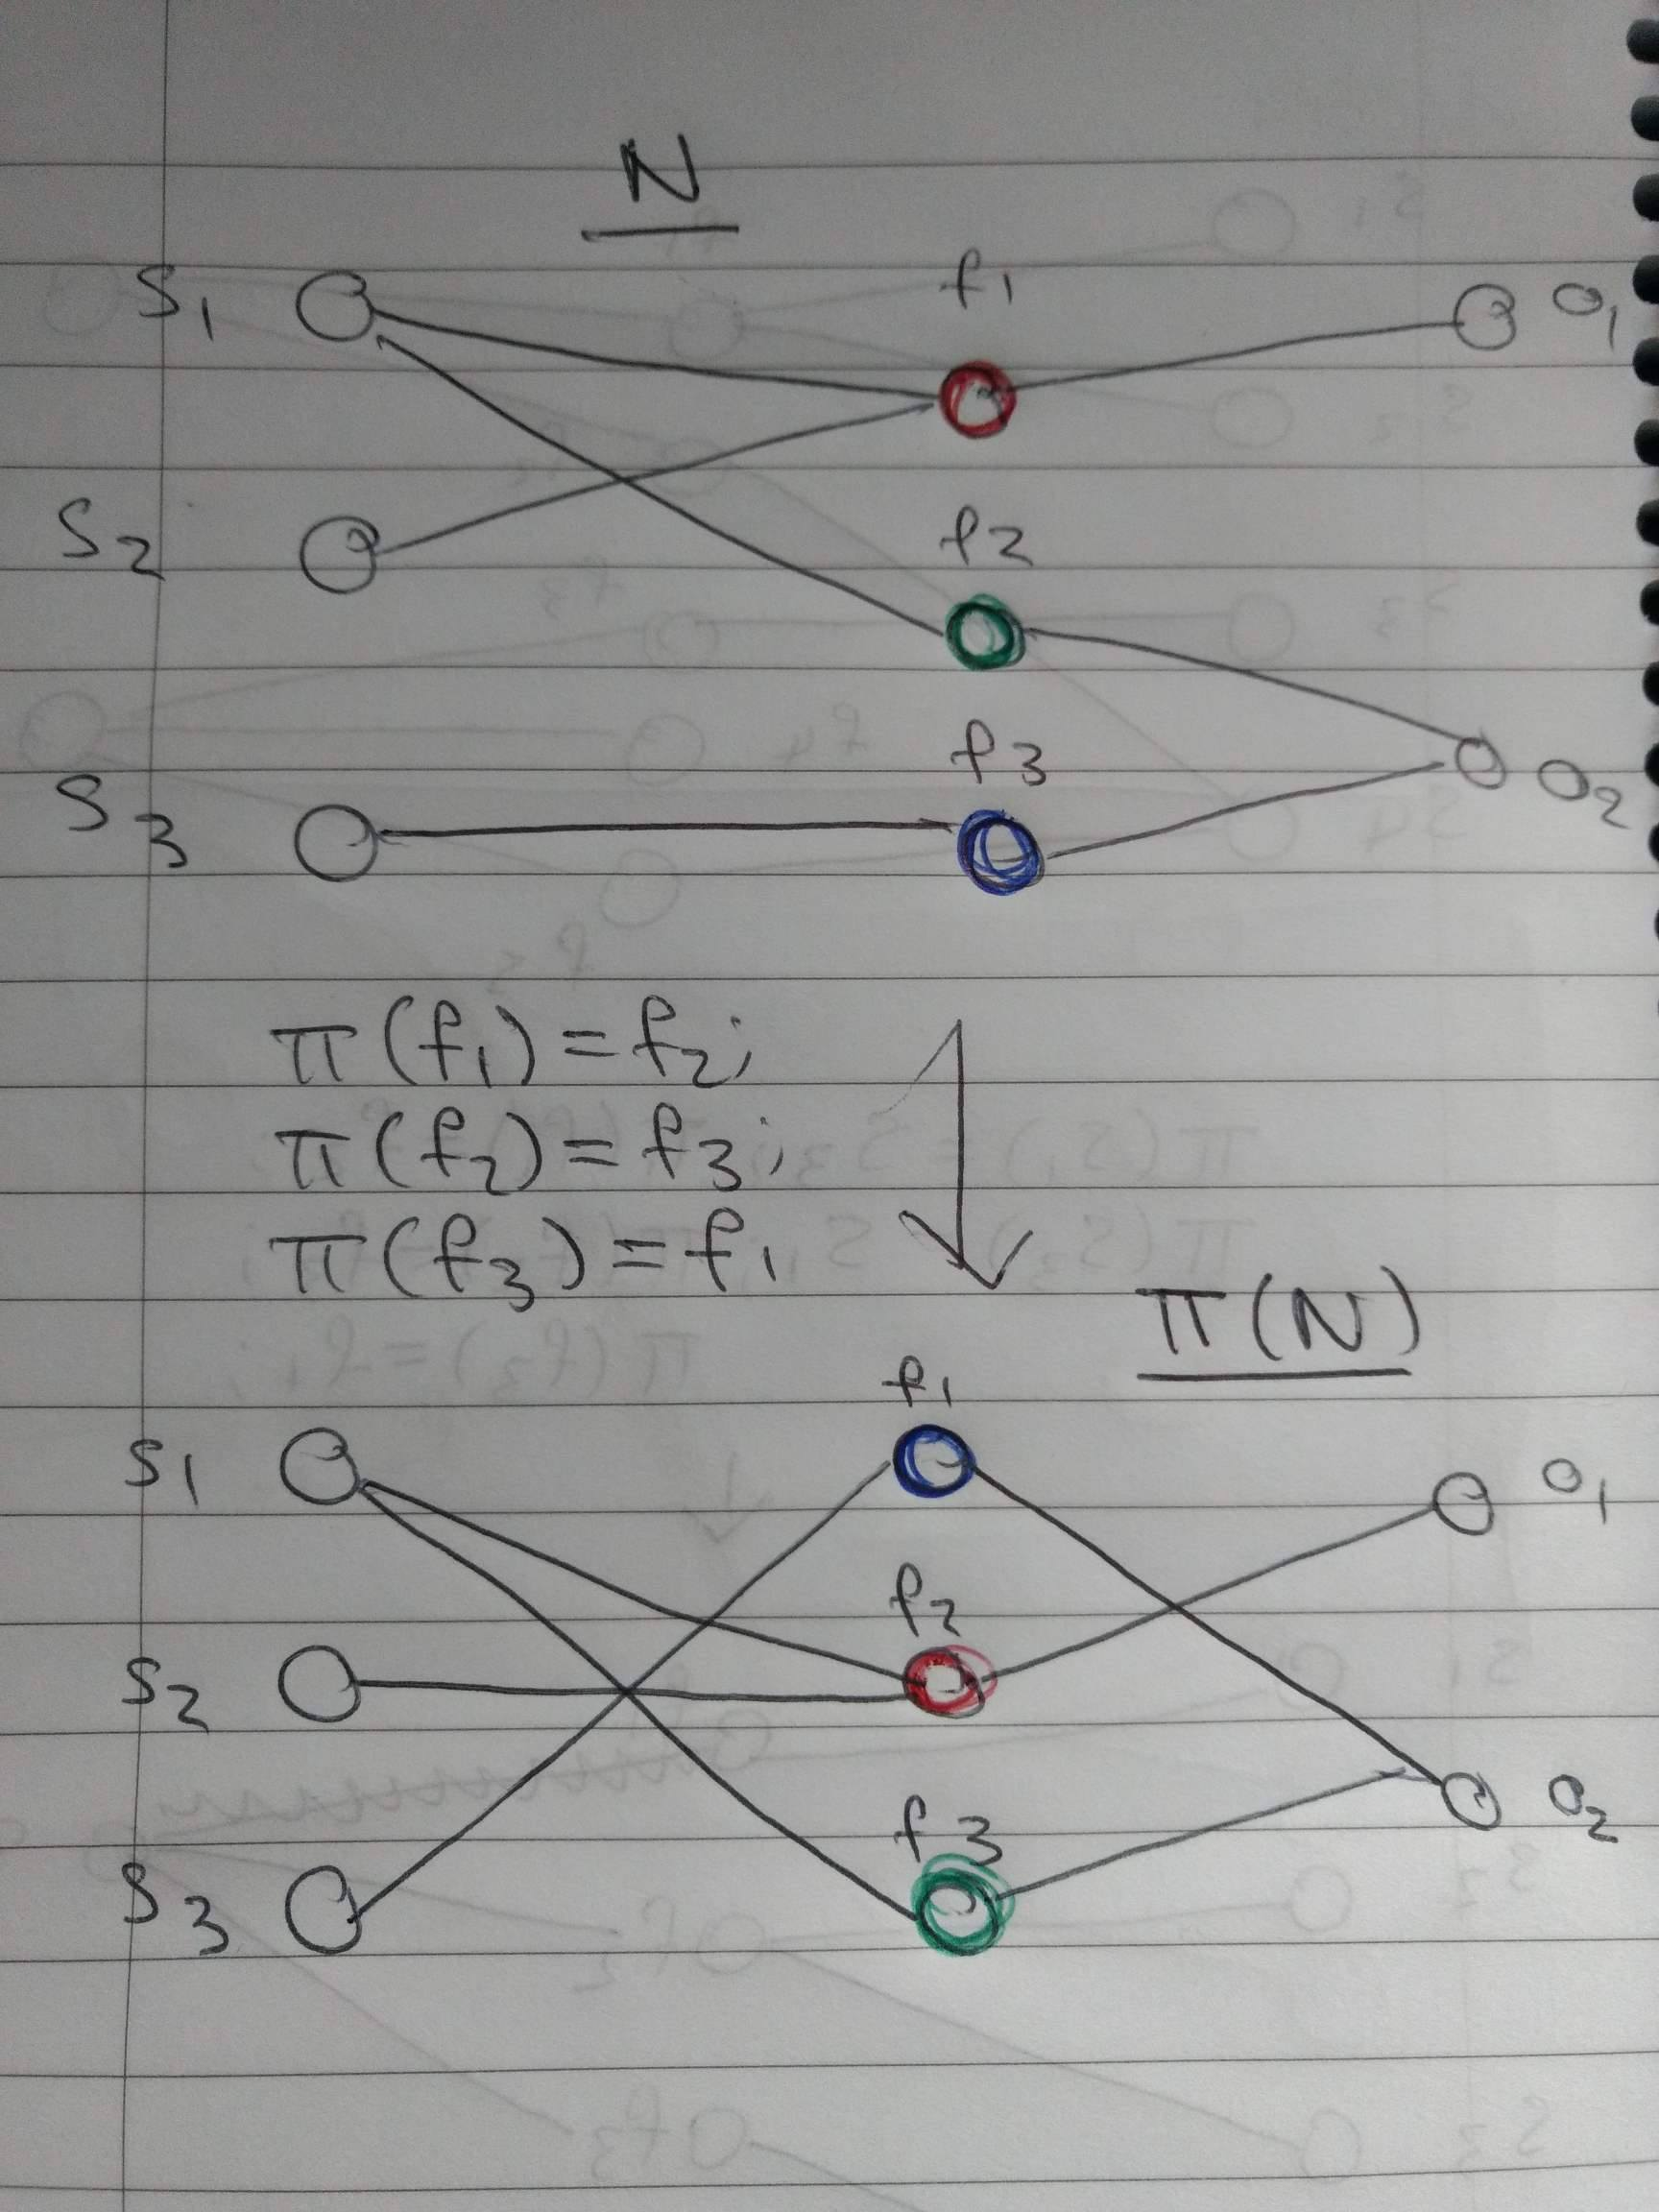
\includegraphics[width=\linewidth]{symmetry_example}
    \captionof{figure}{Example of a permutation of a truth-discovery network}
    \label{img:permutation_of_a_tdn}
}

\bibliography{references}{}
\bibliographystyle{plain}

% \end{multicols}
\end{document}
